\section{Resumo}



\clearpage

\section{Motivação}


\begin{figure}[H]
	\centering
	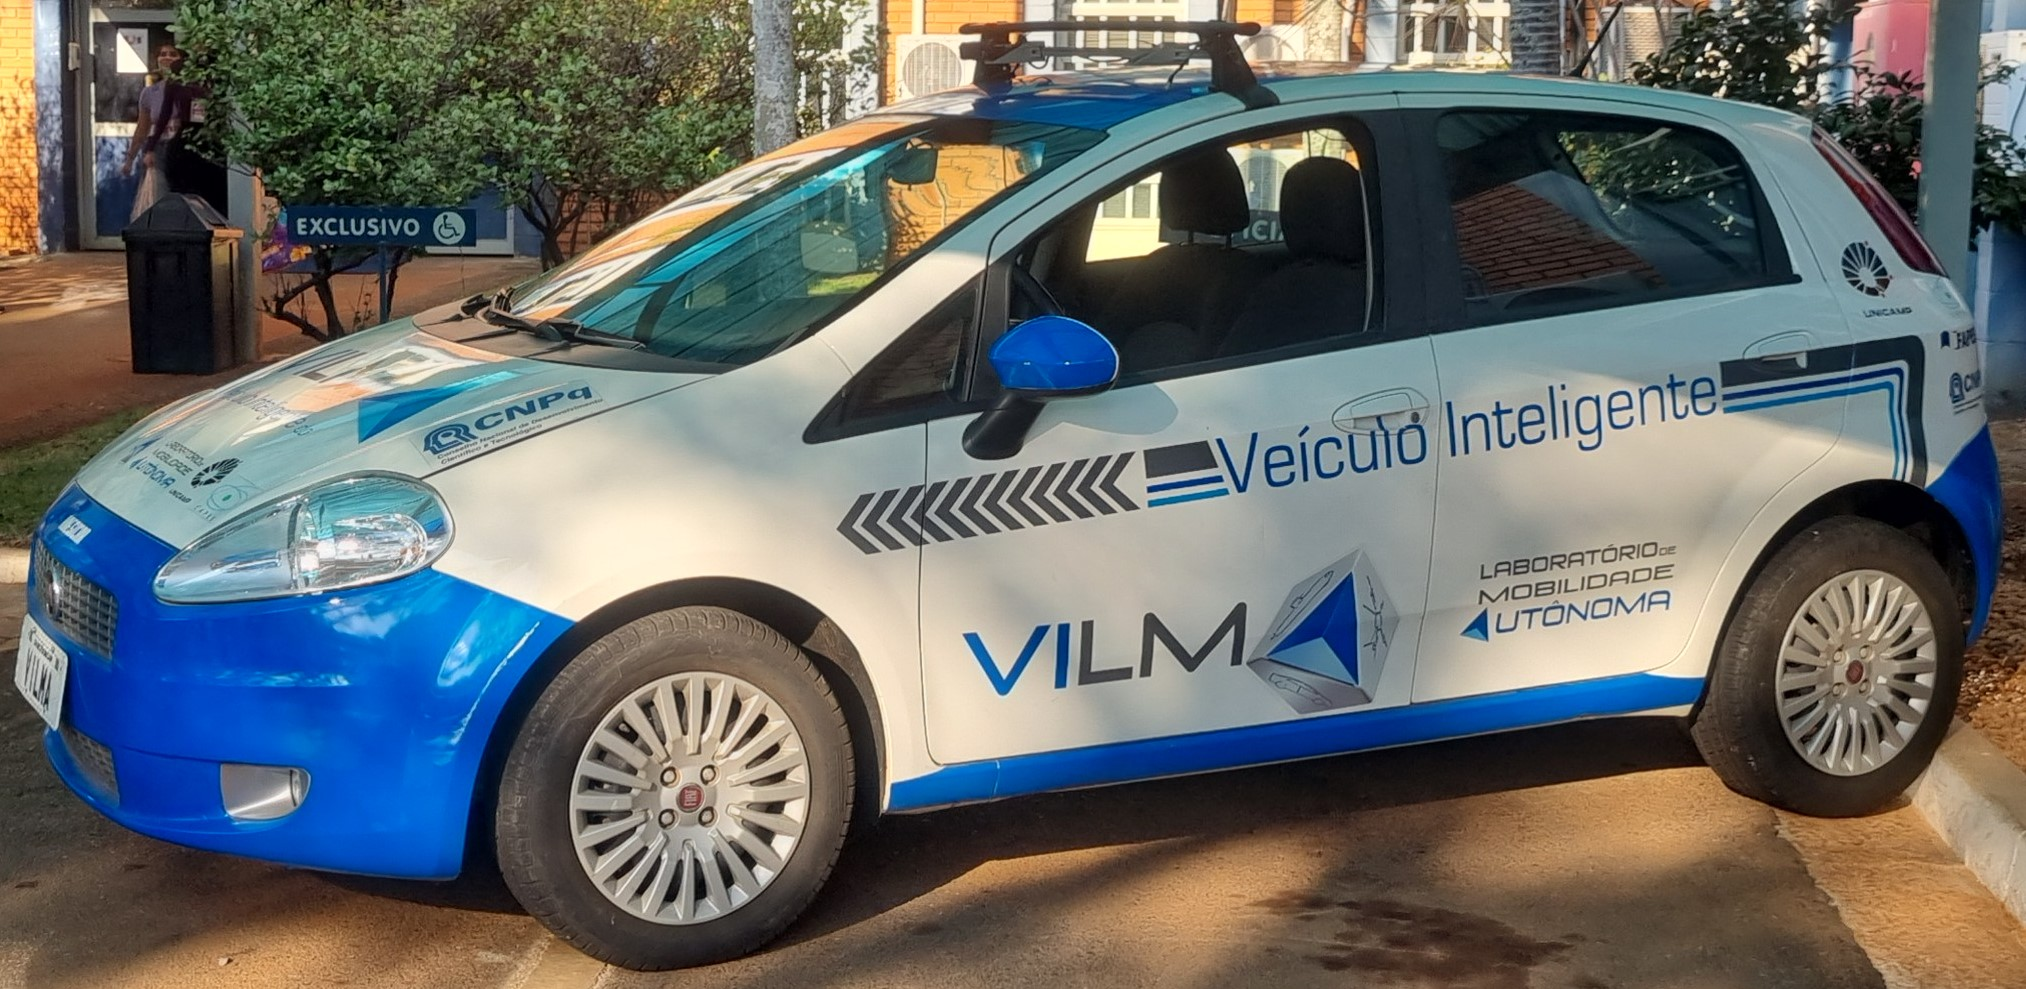
\includegraphics[width=0.5\linewidth]{img/vilma}
	\caption{Veículo Autônomo do LMA.}
	\label{fig:vilma}
\end{figure}

\begin{figure}[H]
	\centering
	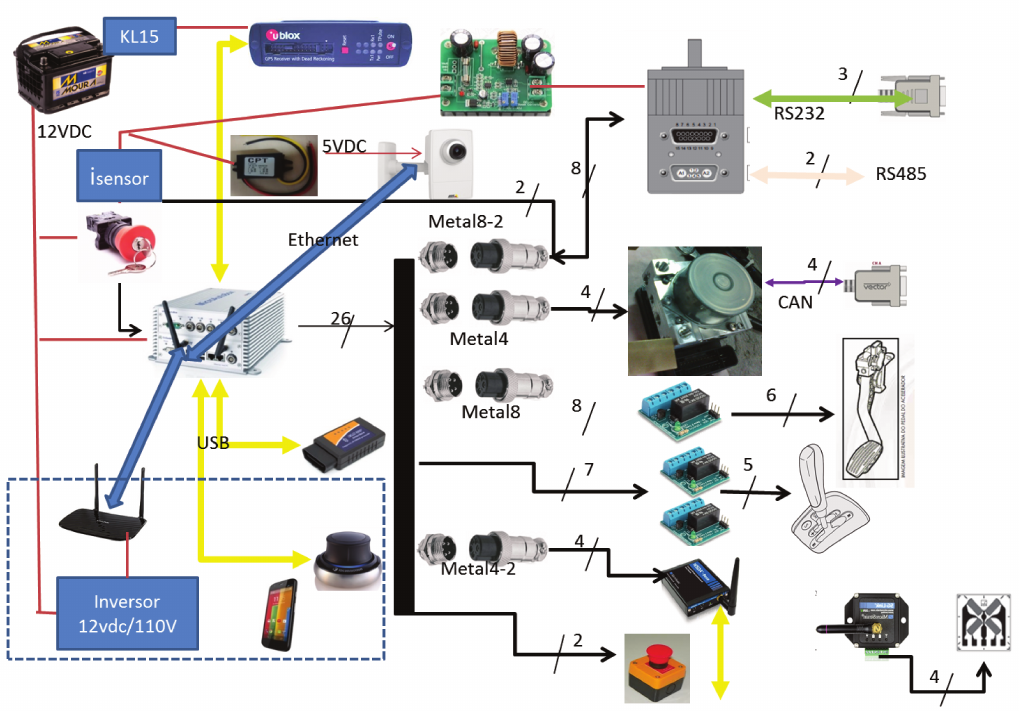
\includegraphics[width=0.75\linewidth]{img/diagrama_vilma}
	\caption{Diagrama de \textit{hardware} do VILMA01 \cite{bedoya_alise_2016}.}
	\label{fig:diagrama_vilma}
\end{figure}

\begin{figure}
	\centering
	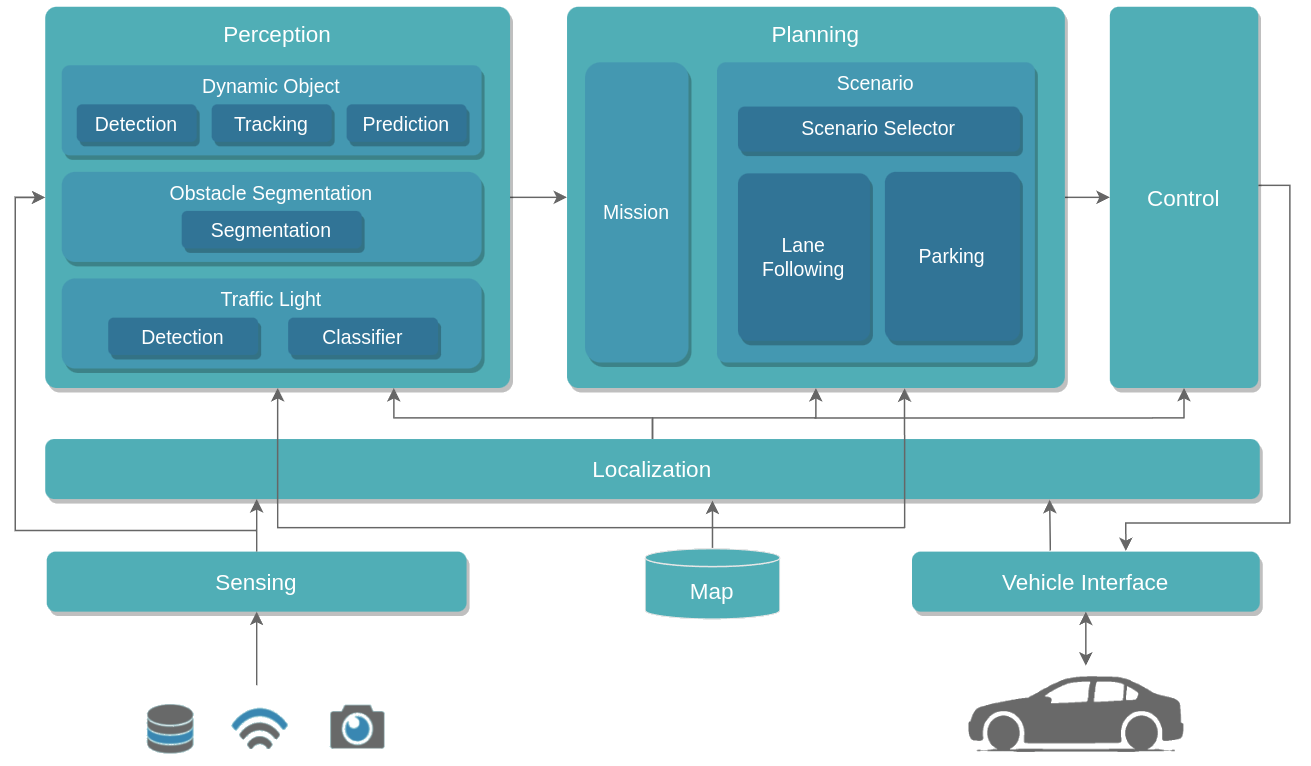
\includegraphics[width=0.8\linewidth]{img/HL_architecture}
	\caption{Arquitetura de alto nível \cite{autowareArchitecture}.}
	\label{fig:hlarchitecture}
\end{figure}


\clearpage

\section{Documentação}

\begin{figure}[H]
	\centering
	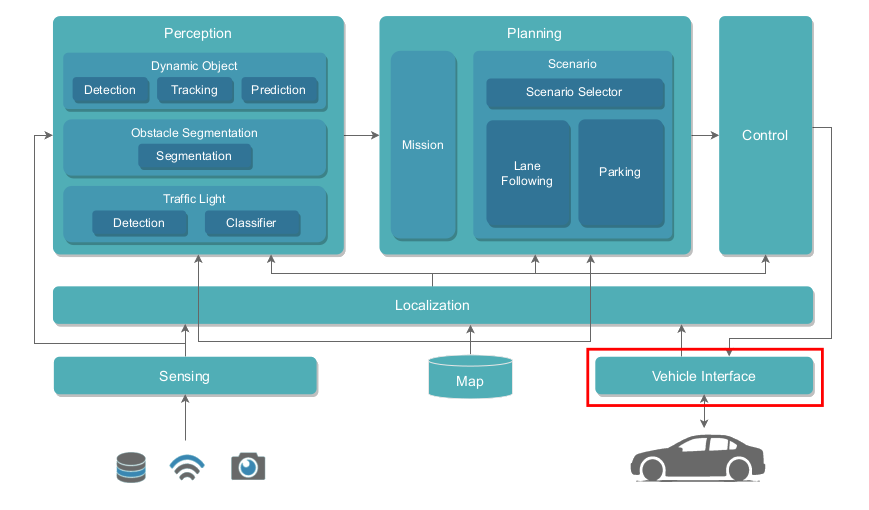
\includegraphics[width=0.75\linewidth]{img/architecture.png}
	\caption{Escopo do projeto na arquitetura Autoware.}
	\label{fig:architecture}
\end{figure}

\begin{figure}[H]
	\centering
	\includegraphics[width=0.55\linewidth]{img/architecture_HIL}
	\caption{Arquitetura de teste do \textit{hardware}.}
	\label{fig:architecture_HIL}
\end{figure}

	\begin{figure}[H]
	\centering
	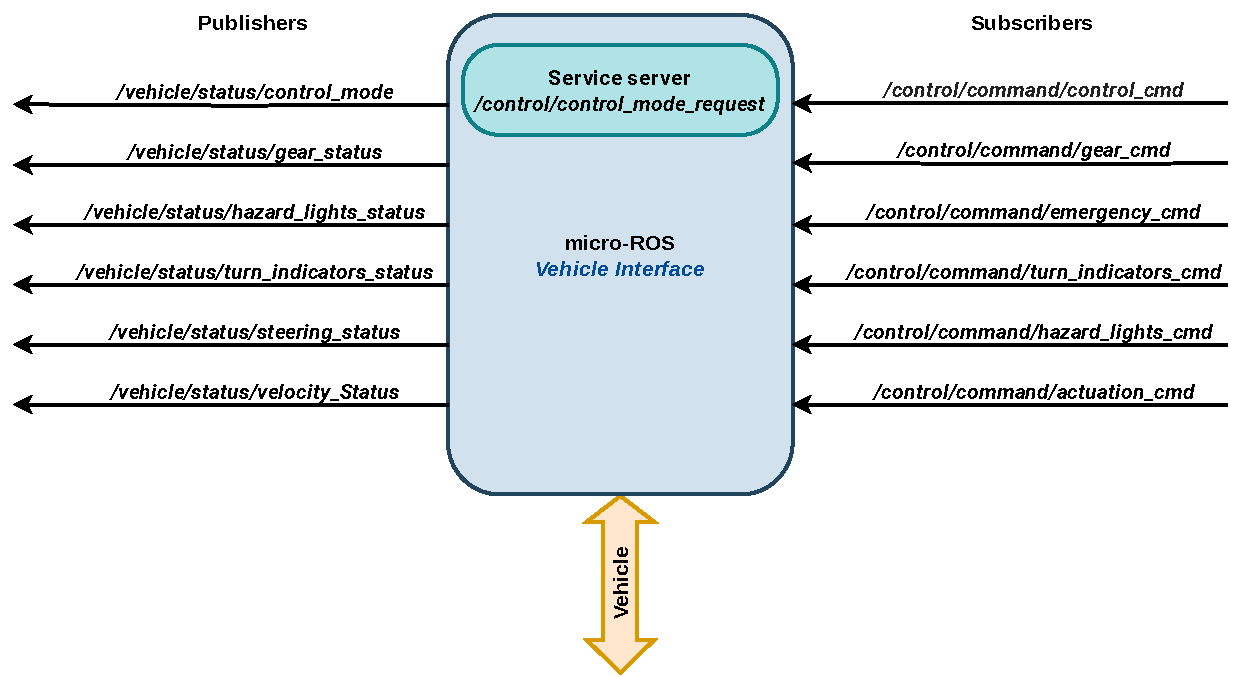
\includegraphics[width=0.75\linewidth]{img/vehicle_interface-topics}
	\caption{Diagrama de tópicos da \textit{vehicle interface}.}
	\label{fig:vehicleinterface-topics}
\end{figure}

\subsection{Requisitos}

\subsubsection*{Requisitos funcionais}
	
	\begin{itemize}
		\item Comunicação com o Autoware;
		\item Controle da aceleração, frenagem e direção do veículo;
		\item Controle dos faróis e luzes de sinalização (seta) do veículo;
		\item Teleoperação do veículo por um \textit{joystick} em  \textit{hardware};
		\item Troca do modo de operação por meio da \textit{switch} do \textit{joystick};
		\item Subscrição por meio do micro-ROS em todos os tópicos necessários do Autoware;
		\item Publicação a partir micro-ROS em todos os tópicos necessários do Autoware.
		
	\end{itemize}

\subsubsection*{Requisitos não funcionais}
	
	\begin{itemize}
		\item A \textit{vehicle interface} deve ser construída na forma de um pacote portável para outros microcontroladores STM32;
		\item O interfaceamento com o veículo deve ser intercambiável com diferentes configurações;
		\item Deve-se garantir sincronização de \textit{timestamp} entre o Autoware e o microcontrolador;
		\item O sistema embarcado deve abstraír o veículo como um sistema \textit{Drive-By-Wire} (DBW) para o Autoware.
	\end{itemize}
	
\subsection{Componentes}

\subsubsection*{Placa de desenvolvimento NUCLEO-H753ZI}
	
	\begin{itemize}
		\item Microcontrolador STM32H753ZI;
		\item ARM Cortex-M7;
		\item 1 MB RAM;
		\item 2 MB Flash;
		\item \textit{Clock} máximo de 480 MHz;
		\item DMA;
		\item Comunicação:
		\begin{itemize}
			\item UART/USART;
			\item Ethernet;
			\item USB.
		\end{itemize}
		\item Custo: US\$ 27,00.
	\end{itemize}

\begin{figure}[H]
	\centering
	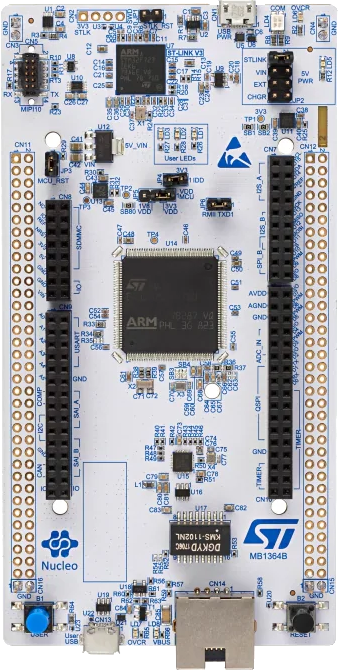
\includegraphics[width=0.25\linewidth]{img/nucleo}
	\caption{NUCLEO-753ZI.}
	\label{fig:nucleo}
\end{figure}

\subsubsection*{Joystick}
	
	\begin{itemize}
		\item Tensão de operação: 3V3 -- 5V;
		\item Saída analógica referente ao eixo $x$;
		\item Saída analógica referente ao eixo $y$;
		\item Saída digital referente ao eixo $z$;
		\item Custo: R\$ 10,00.
	\end{itemize}

\begin{figure}[H]
	\centering
	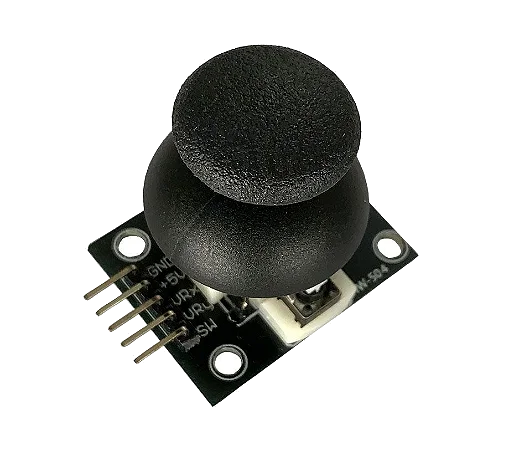
\includegraphics[width=0.3\linewidth]{img/joystick}
	\caption{Joystick 2 eixos.}
	\label{fig:joystick}
\end{figure}

\subsection{Arquitetura}

\begin{figure}[H]
	\centering
	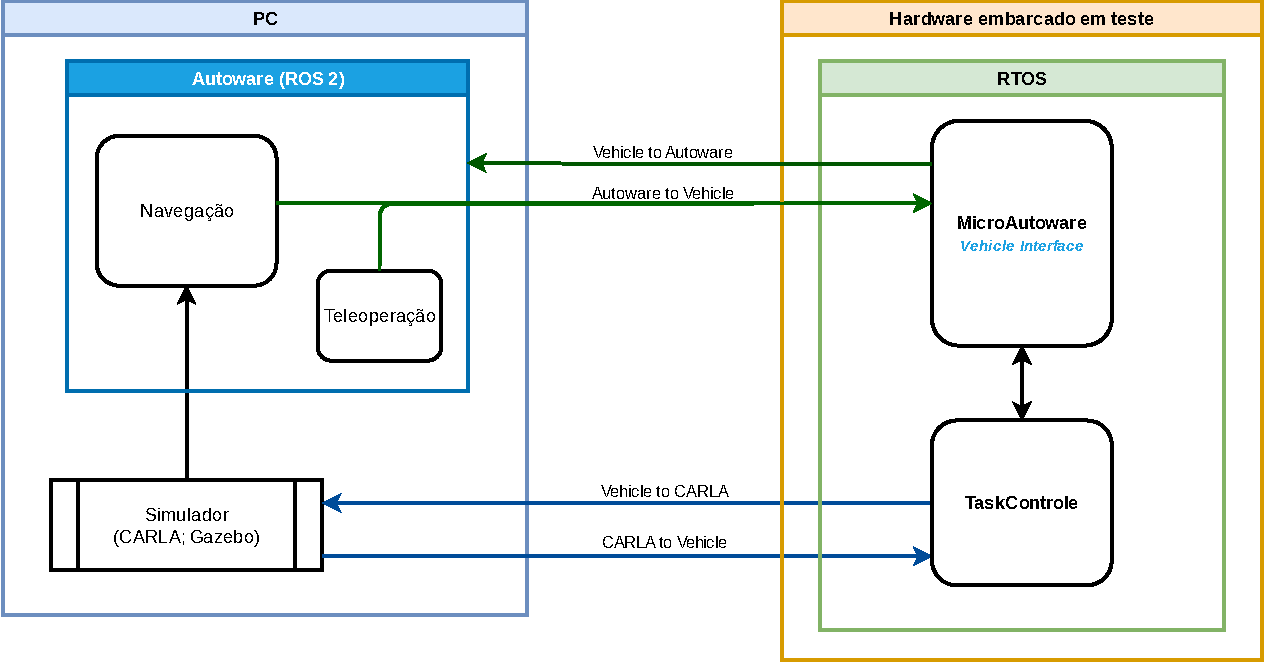
\includegraphics[width=0.75\linewidth]{img/highLevelblock_diagram.pdf}
	\caption{Diagrama de blocos em alto nível da arquitetura HIL.}
	\label{fig:highLevelblock_diagram}
\end{figure}

\begin{figure}[H]
	\centering
	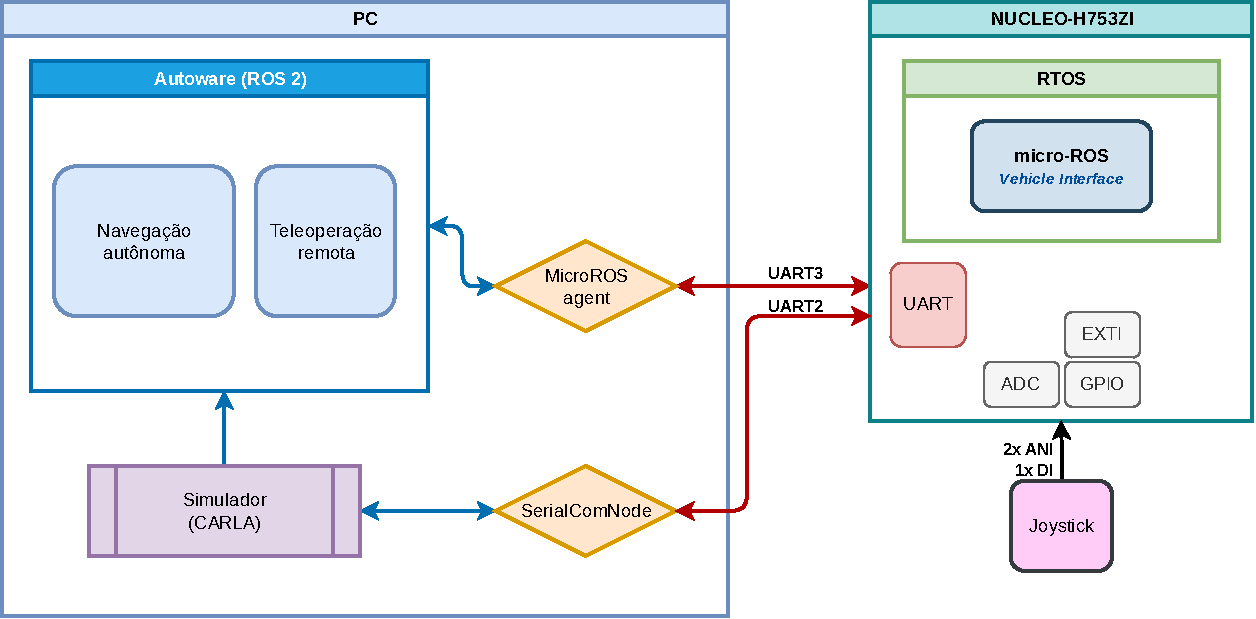
\includegraphics[width=0.75\linewidth]{img/block_diagram.pdf}
	\caption{Diagrama de blocos do sistema embarcado.}
	\label{fig:blockdiagram}
\end{figure}

\begin{figure}[H]
	\centering
	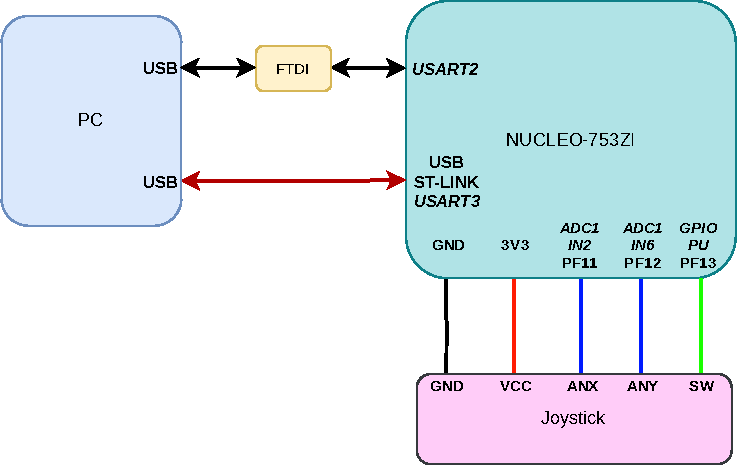
\includegraphics[width=0.6\linewidth]{img/esquematico.pdf}
	\caption{Esquemático de ligações elétricas.}
	\label{fig:esquematico}
\end{figure}

\subsubsection*{Periféricos}

\begin{itemize}
	\item \textit{Direct Memory Access}
	\begin{itemize}
		\item DMA1
		
		\item DMA2		
	\end{itemize}
	
	\item UART
	\begin{itemize}
		\item USART3
		
		\item USART2
		
	\end{itemize}
	
	\item ADC
	
	\item EXTI
	
	
	
\end{itemize}


\subsection{Método de desenvolvimento}


\begin{figure}[H]
	\centering
	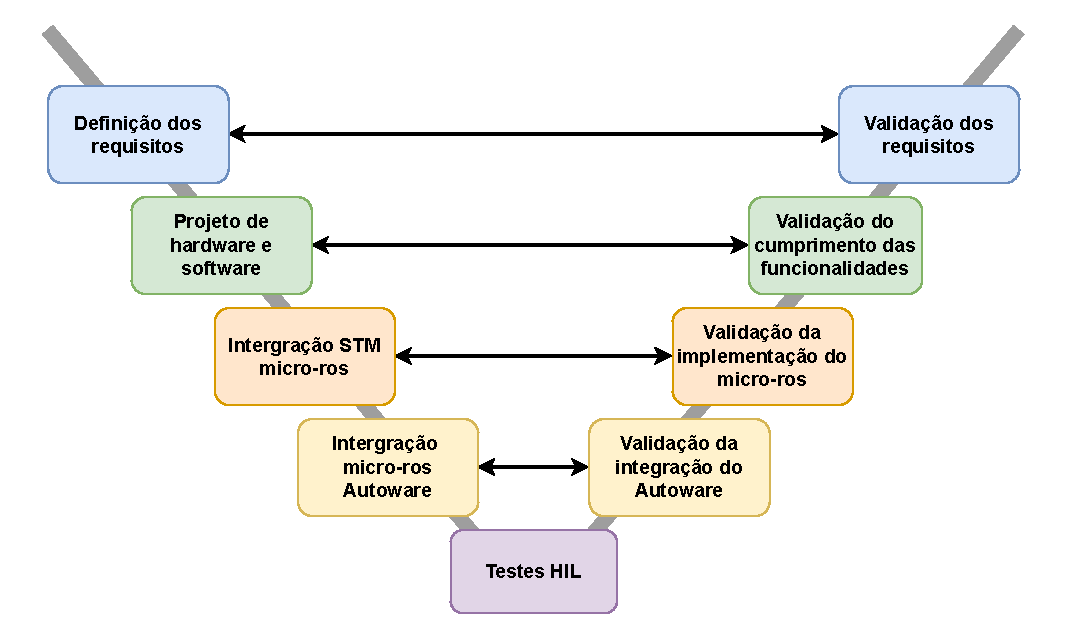
\includegraphics[width=0.75\linewidth]{img/modelo-v}
	\caption{Modelo de execução das atividades do projeto.}
	\label{fig:modelo-v}
\end{figure}

\begin{table}[H]
	\centering
	\small{
		\begin{tabular}{|c|c|c|c|c|c|c|c|c|c|}
			\hline
			\textbf{Atividade/Semana} & 1 & \textbf{2} & 3 & \textbf{4} & 5 & 6 & \textbf{7} & 8 & \textbf{9} \\
			\hline
			Proposta do projeto  & \cellcolor{unifeiblue} &  &  &  &  &  &  &  &  \\
			\hline
			Projeto de \textit{hardware} e \textit{software}  &  & \cellcolor{unifeiblue} & \cellcolor{unifeiblue} &  &  &  &  &  &  \\
			\hline
			Integração do STM com o micro-ROS  &  & \cellcolor{unifeiblue} &  &  &  &  &  &  &  \\
			\hline
			Integração do micro-ROS com o Autoware  &  &  & \cellcolor{unifeiblue} & \cellcolor{unifeiblue} & \cellcolor{unifeiblue} &  &  &  &  \\
			\hline
			Implementação das tarefas do sistema embarcado  &  &  &  & \cellcolor{unifeiblue} & \cellcolor{unifeiblue} & \cellcolor{unifeiblue} & \cellcolor{unifeiblue} &  &  \\
			\hline
			Construção do ambiente de testes  &  &  &  &  & \cellcolor{unifeiblue} & \cellcolor{unifeiblue} & \cellcolor{unifeiblue} &  &  \\
			\hline
			Realização dos testes  &  &  &  &  &  &  & \cellcolor{unifeiblue} & \cellcolor{unifeiblue} & \cellcolor{unifeiblue} \\
			\hline
			Escrita do relatório  &   & \cellcolor{unifeiblue} & \cellcolor{unifeiblue} & \cellcolor{unifeiblue} & \cellcolor{unifeiblue} & \cellcolor{unifeiblue} & \cellcolor{unifeiblue} & \cellcolor{unifeiblue} & \cellcolor{unifeiblue} \\
			\hline
		\end{tabular}
	}
	\caption{Cronograma de atividades.}
	\label{tab:crono}
\end{table}

\begin{itemize}
	\small
	\item \textbf{Semana 2:} Apresentação Etapa 1
	\item \textbf{Semana 4:} Apresentação Etapa 2
	\item \textbf{Semana 7:} Apresentação Etapa 3
	\item \textbf{Semana 9:} Apresentação Final
\end{itemize}


\subsection{Projeto de \textit{software}}

\subsubsection*{Estados do sistema}

\begin{figure}[H]
	\centering
	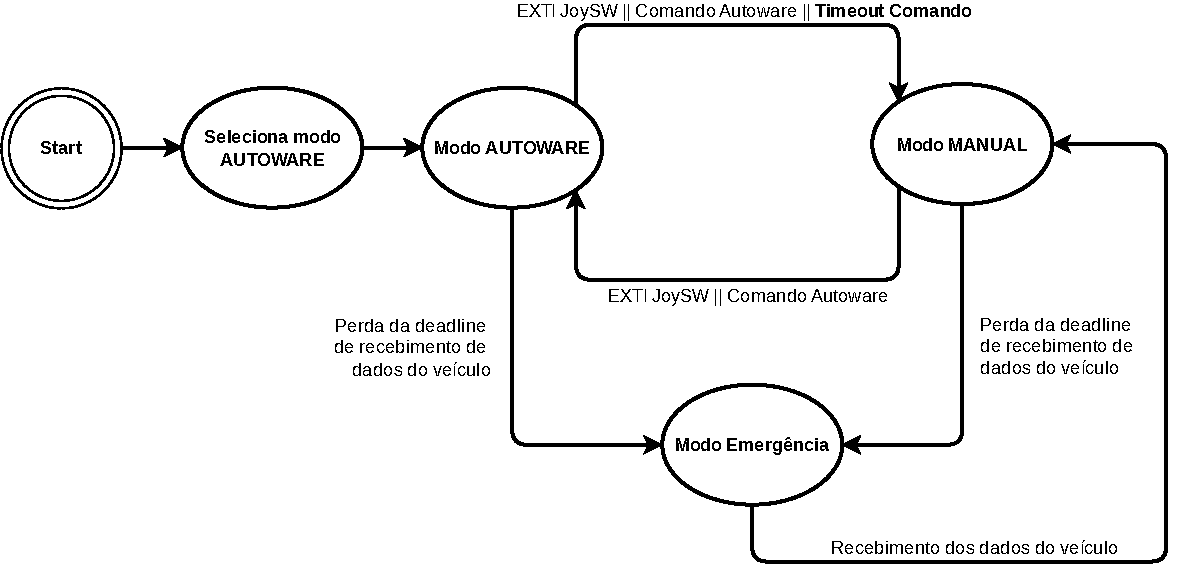
\includegraphics[width = 0.75\textwidth]{img/maquinadeestados}
	\caption{Máquina de estados do sistema.}
	\label{fig:maquinadeestados}
\end{figure}

\subsubsection*{Protocolo de comunicação serial}


\begin{enumerate}
	\item CARLA $\longrightarrow$ RTOS (\texttt{USART3})
	\begin{itemize}
		\item Informações:
		\begin{itemize}
			\item Acelerador, \texttt{float}.
			\item Freio, \texttt{float}.
			\item Esterçamento, \texttt{float}.
			\item Freio de mão, \texttt{unsigned char}.	
			\item Troca de marcha manual, \texttt{unsigned char}.	
			\item Modo reverter, \texttt{unsigned char}.	
			\item Marcha, \texttt{unsigned char}.			
		\end{itemize}
		\item Padrão da mensagem: \texttt{\#T\%c\%c\%c\%cS\%c\%c\%c\%cB\%c\%c\%c\%cH\%cR\%cG\%cM\%c\$}
		
	\end{itemize}
	\item RTOS $\longrightarrow$ CARLA (\texttt{USART2})
	\begin{itemize}
		\item Informações:
		\begin{itemize}
			\item Velocidade longitudinal, \texttt{float}.
			\item Velocidade lateral, \texttt{float}.
			\item Velocidade de guinada, \texttt{float}.
			\item Marcha atual, \texttt{unsigned char}.			
		\end{itemize}
		\item Padrão da mensagem: \texttt{\#A\%c\%c\%c\%cB\%c\%c\%c\%cC\%c\%c\%c\%cD\%c\$}
		
	\end{itemize}
\end{enumerate}


% TODO: \usepackage{graphicx} required
\begin{figure}[H]
	\centering
	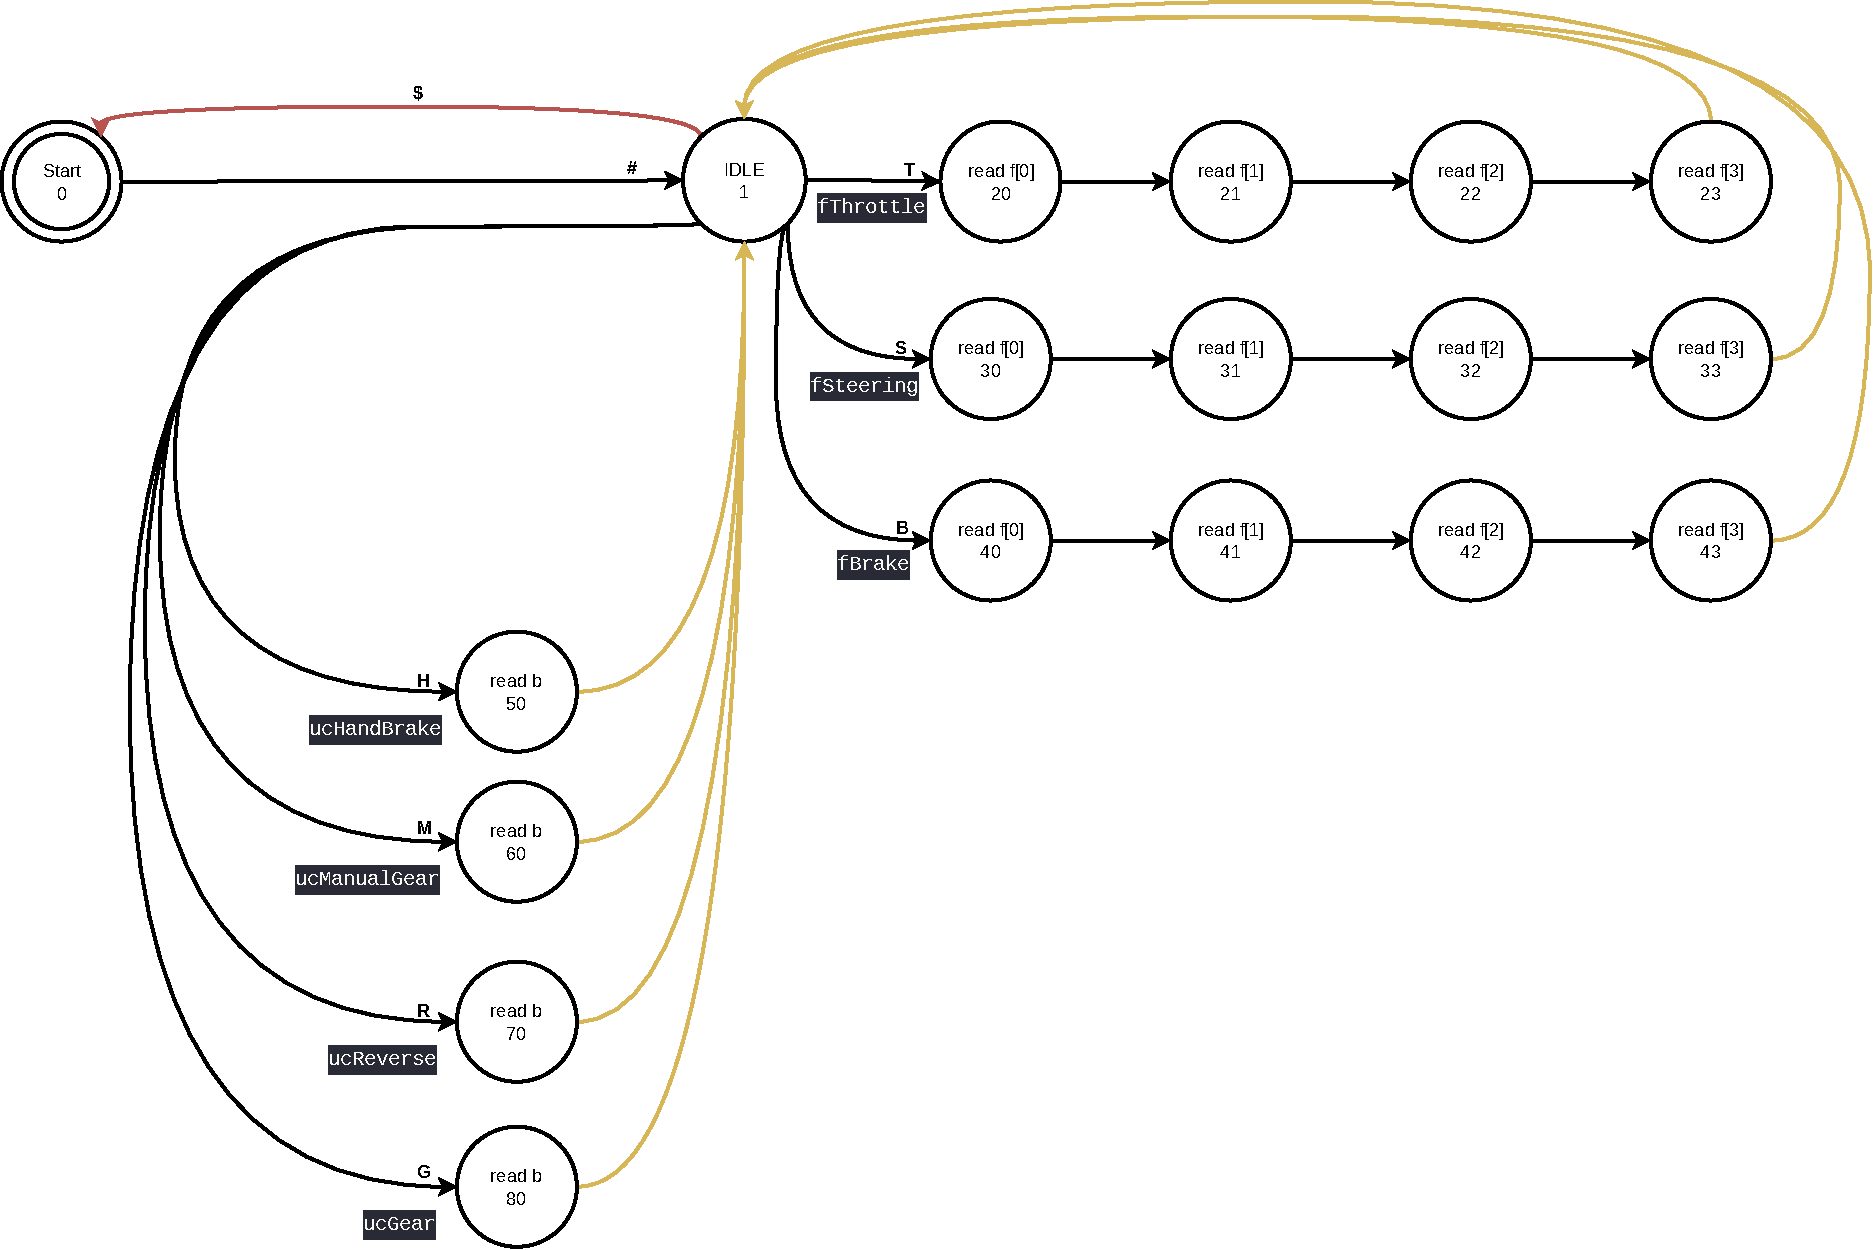
\includegraphics[width=1\linewidth]{img/sm_uc_carla}
	\caption{Máquina de estados da comunicação serial do RTOS para o CARLA.}
	\label{fig:smuccarla}
\end{figure}


% TODO: \usepackage{graphicx} required
\begin{figure}[H]
\centering
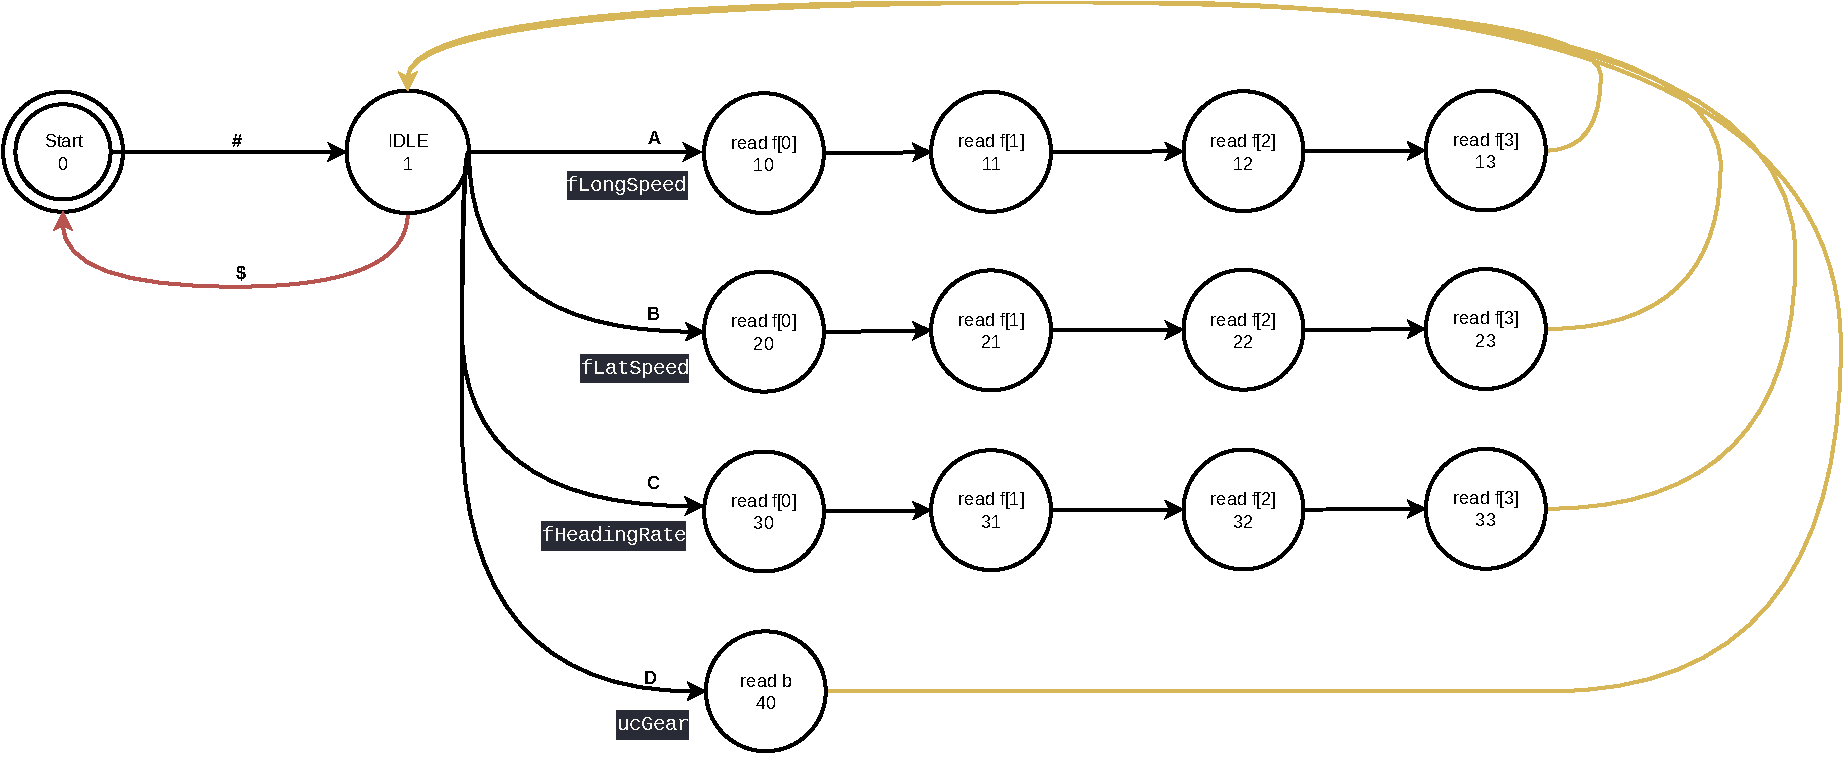
\includegraphics[width=1\linewidth]{img/sm_carla_uc}
\caption{Máquina de estados da comunicação serial do CARLA para o RTOS.}
\label{fig:sm_carla_uc}
\end{figure}



\subsubsection*{Tarefas}

\begin{figure}[H]
	\centering
	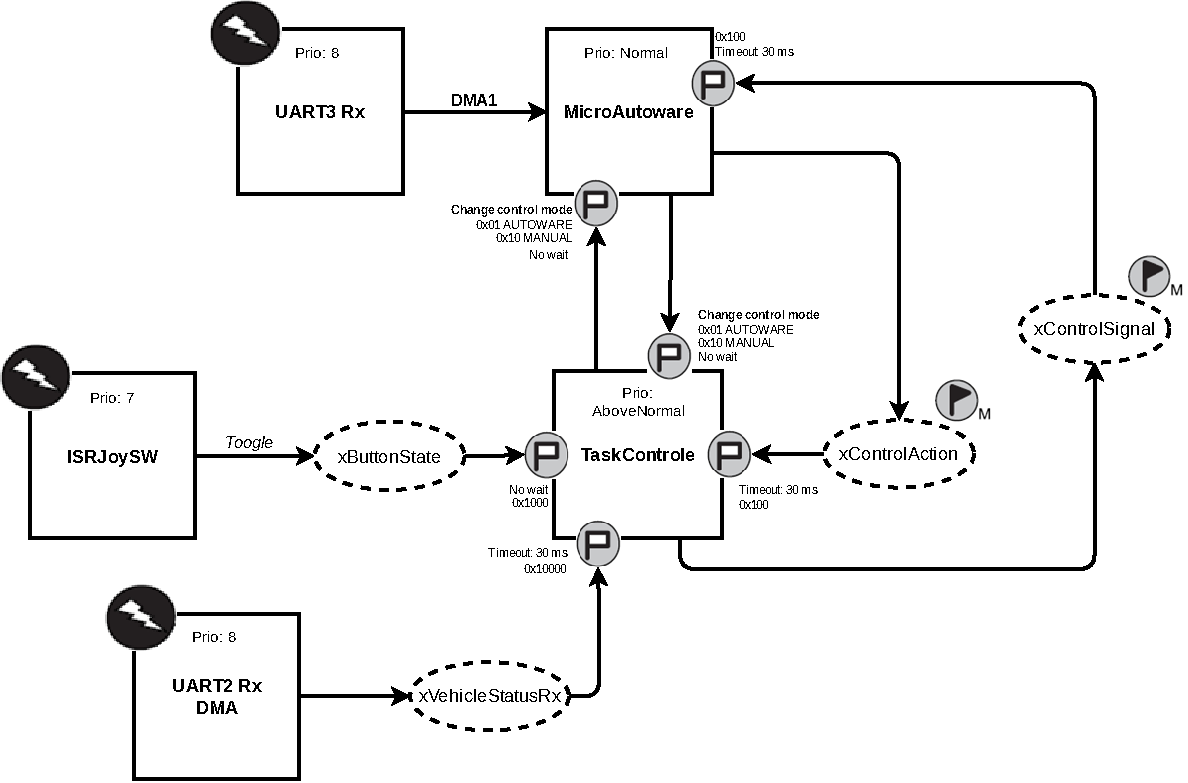
\includegraphics[width = \textwidth]{img/system_diagram}
	\caption{Diagrama do sistema embarcado.}
	\label{fig:systemdiagram}
\end{figure}

\begin{table}[H]
	\centering
	\begin{tabular}{c|p{11.5cm}}
		\textbf{Nome} & MicroAutoware \\
		\hline
		\textbf{Prioridade}& Normal \\
		\hline
		\textbf{Tamanho da stack} & 3500 kB \\
		\hline
		\textbf{Detalhes} & Leitura dos \textit{subscribers} Autoware, leitura dos \textit{subscribers} CARLA, envio das informações de controle e modo de operação para a TaskControle, recebimentos das informações de controle da TaskControle, escrita dos \textit{publishers} Autoware, escrita dos \textit{publishers} CARLA.\\
	\end{tabular}
	\caption{Especificaçõe da tarefa MicroAutoware.}
	\label{tab:microautoware}
\end{table}

\begin{figure}[H]
	\centering
	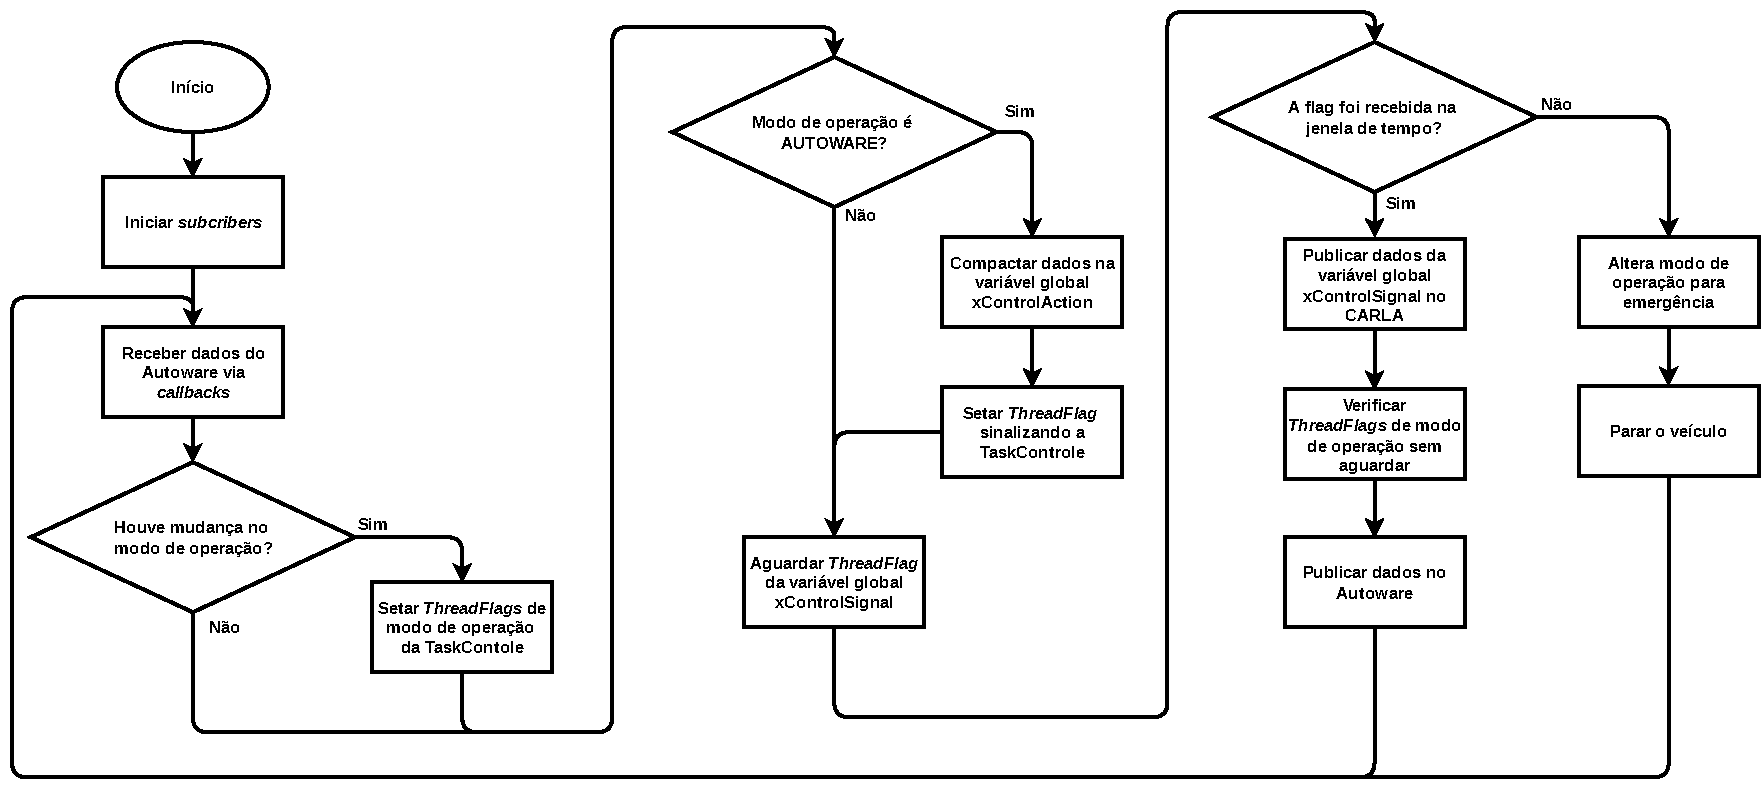
\includegraphics[width = \textwidth]{img/fluxograma_microautoware}
	\caption{Fluxograma da tarefa MicroAutoware.}
	\label{fig:fluxograma_microautoware}
\end{figure}

\begin{table}[H]
	\centering
	\begin{tabular}{c|p{11.5cm}}
	\textbf{Nome} & TaskControle \\
	\hline
	\textbf{Prioridade}& AboveNormal \\
	\hline
	\textbf{Tamanho da stack} & 500 kB \\
	\hline
	\textbf{Detalhes} & Realiza o controle do veículo utilizando a referência dada pelo \textit{joystick} ou pelo Autoware, dado o modo de operação, podendo ser MANUAL ou AUTOWARE, respectivamente. A alteração do modo é feita por \textit{ThreadFlag}, gerada por ISR ou pelo Autoware. Em caso do modo de operação AUTOWARE, os sinais de controle são recebidos por variável global e sincronizados por \textit{ThreadFlag}, com tempo de 30 ms, onde caso não receba, entra em algum modo de segurança. Em caso de operação MANUAL,  o \textit{joystick} é lido por DMA, aguardando 20 ms antes de cada leitura,  convertendo os valores analógicos em sinais de controle, onde também caso haja algum erro, o modo de emergência é acionado. O sinal de controle é enviado para o MicroAutoware por uma variável global e sincronizado por \textit{ThreadFlag}. 
	\end{tabular}
	\caption{Especificaçõe da tarefa TaskControle.}
	\label{tab:taskcontrole}
\end{table}

\begin{figure}[H]
	\centering
	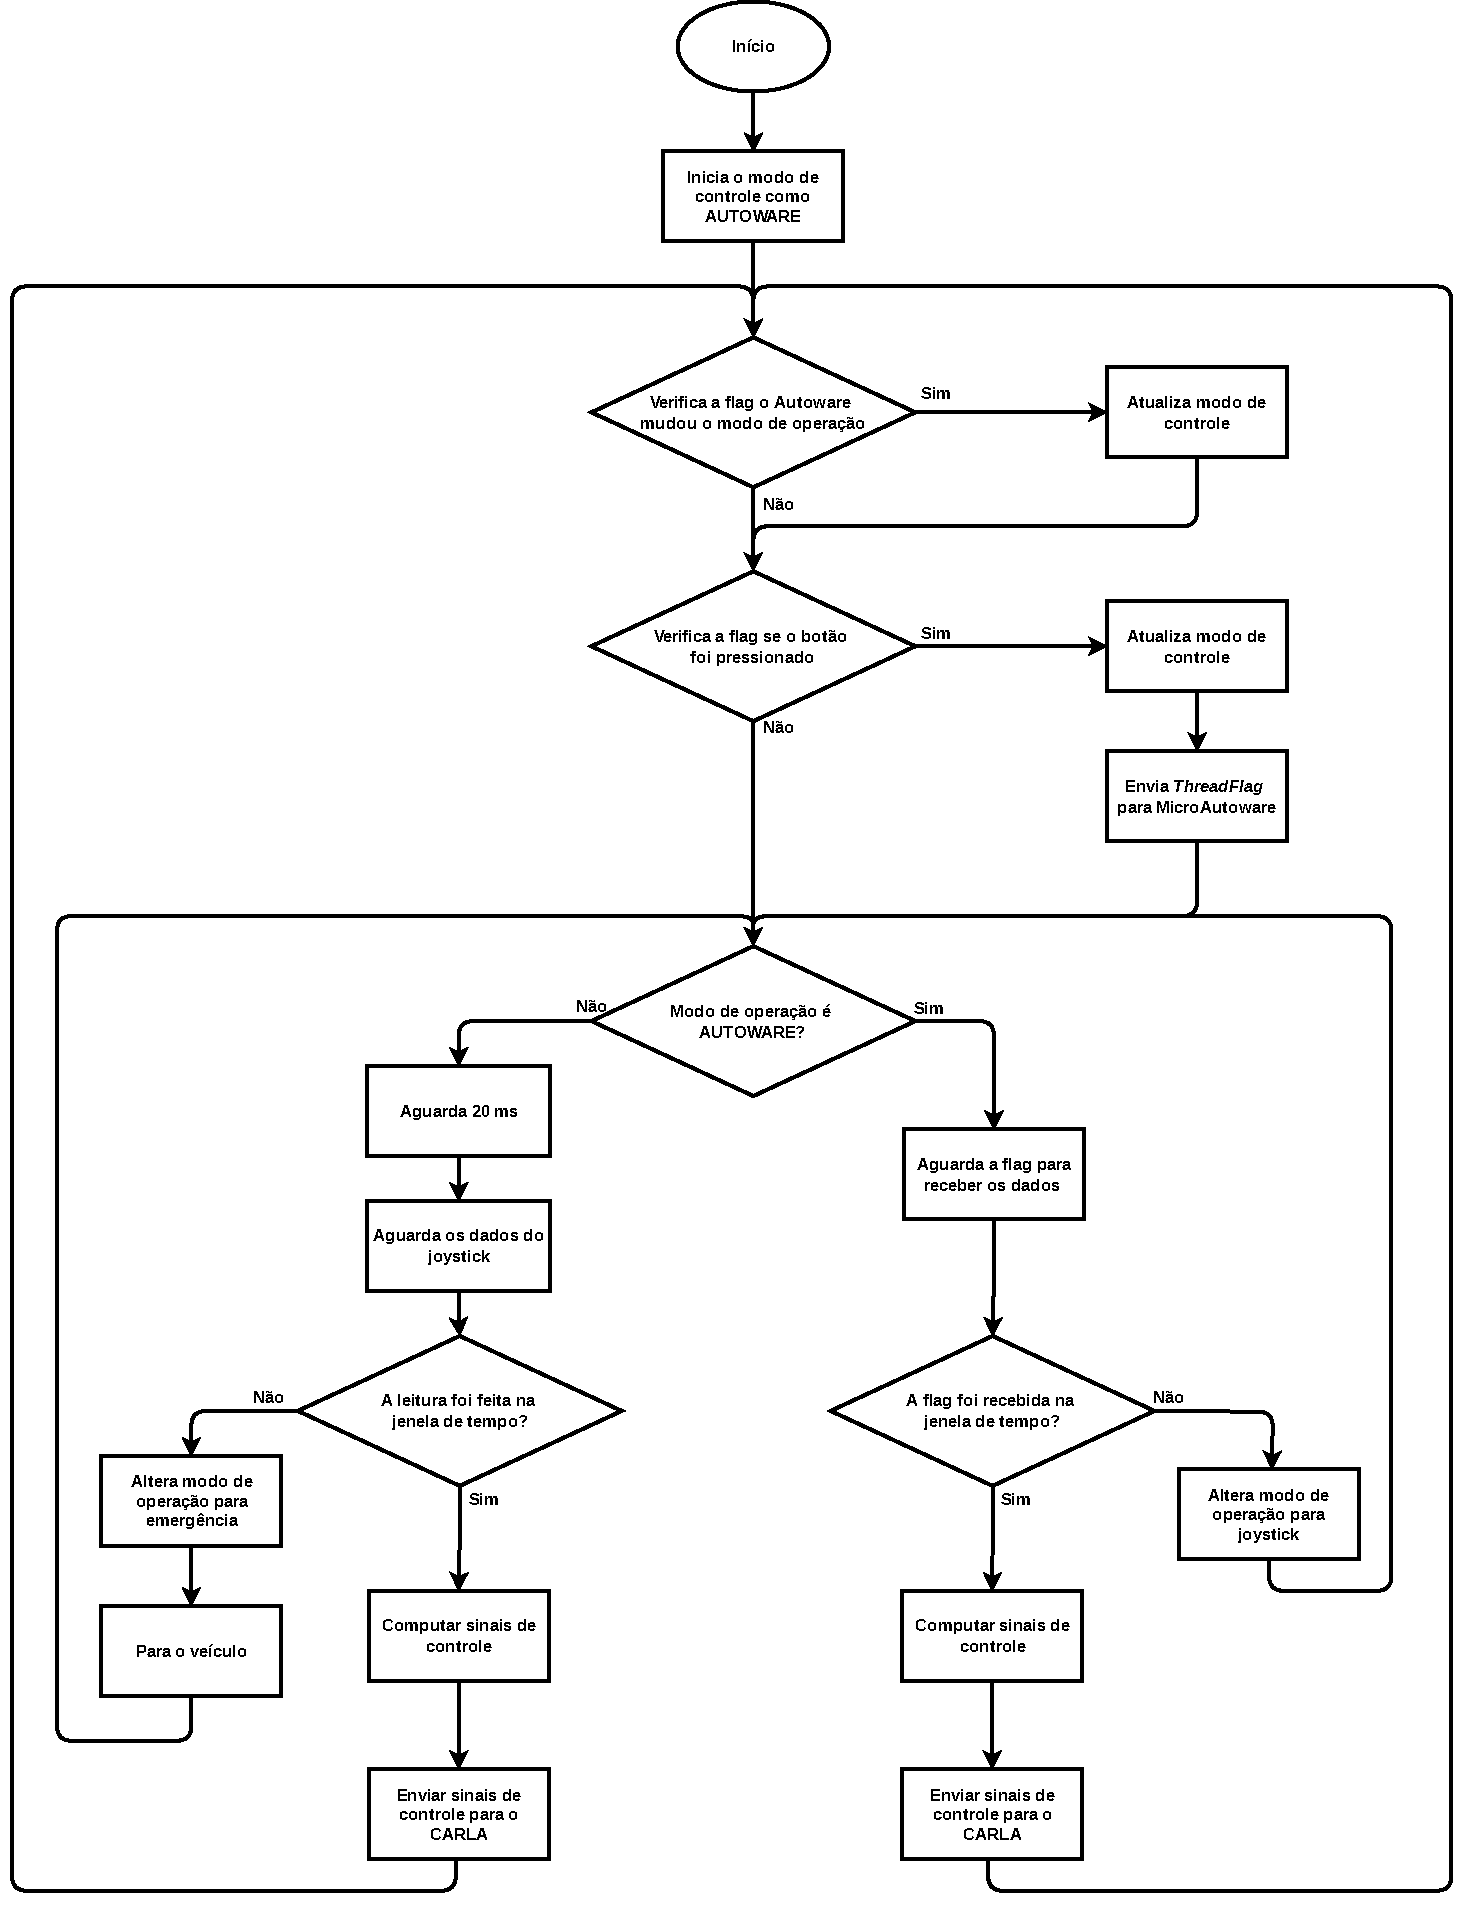
\includegraphics[height= 0.8\textheight]{img/fluxograma_taskcontrole}
	\caption{Fluxograma da tarefa TaskControle.}
	\label{fig:fluxograma_taskcontrole}
\end{figure}


\begin{figure}[H]
	\centering
	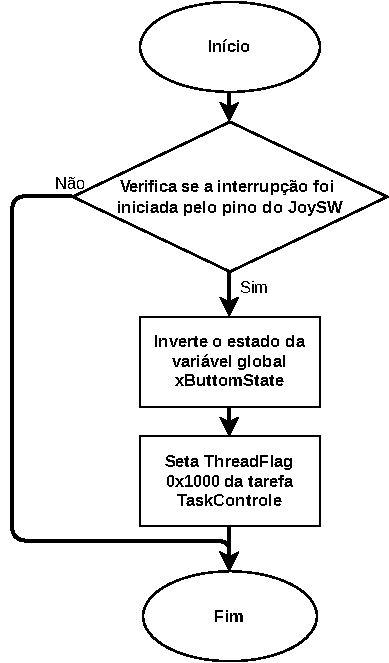
\includegraphics[height= 0.3\textheight]{img/fluxograma_joysw}
	\caption{Fluxograma da ISR JoySW.}
	\label{fig:fluxograma_joysw}
\end{figure}

\subsubsection*{Sinalização \texttt{xButtonState}}
	
	\begin{itemize}
		\item \textbf{Objeto:} \textit{ThreadFlag}
		\item \textbf{Flag:} 0x1000
		\item \textbf{Modo:} \textit{No wait}
		\item \textbf{Descrição:} Sinaliza ocorrência da interrupção do botão JoySW.
		
	\end{itemize}


\subsubsection*{Sinalização \texttt{xControlAction}}
	
	\begin{itemize}
		\item \textbf{Objeto:} \textit{ThreadFlag}
		\item \textbf{Flag:} 0x0100
		\item \textbf{Modo:} \textit{Timeout} 30 ms
		\item \textbf{Descrição:} Sinaliza o recebimento de dados pela variável global \texttt{xControlAction}.
		
	\end{itemize}	

\subsubsection*{Sinalização \texttt{xControlSignal}}
	
	\begin{itemize}
		\item \textbf{Objeto:} \textit{ThreadFlag}
		\item \textbf{Flag:} 0x0100
		\item \textbf{Modo:} \textit{Timeout} 30 ms
		\item \textbf{Descrição:} Sinaliza o recebimento de dados pela variável global \texttt{xControlSignal}.
		
	\end{itemize}	



\subsubsection*{Alteração do modo de condução por interrupção JoySW}
	
	\begin{itemize}
		\item \textbf{Objeto:} \textit{ThreadFlag}
		\item \textbf{Flags:}
		\begin{itemize}
			\item Modo de controle alterado para AUTOWARE: 0x01
			\item Modo de controle alterado para MANUAL: 0x10
			
		\end{itemize}
		\item \textbf{Modo:} \textit{No wait}
		\item \textbf{Descrição:} Realiza a sincronização do modo de operação da tarefa TaskControle para a MicroAutoware.
		
	\end{itemize}

\subsubsection*{Alteração do modo de condução pelo Autoware}
	
	\begin{itemize}
		\item \textbf{Objeto:} \textit{ThreadFlag}
		\item \textbf{Flags:}
		\begin{itemize}
			\item Modo de controle alterado para AUTOWARE: 0x01
			\item Modo de controle alterado para MANUAL: 0x10
			
		\end{itemize}
		\item \textbf{Modo:} \textit{No wait}
		\item \textbf{Descrição:} Realiza a sincronização do modo de operação da tarefa MicroAutoware para a TaskControle.
		
	\end{itemize}


\subsubsection*{Proteção de recursos}



\noindent {Variável global \texttt{xControlSignal}}
	
	\begin{itemize}
		\item Protegida por MUTEX.
		\begin{itemize}
			\item \texttt{MutexControlSignal}
			
		\end{itemize}
	\end{itemize}



\noindent {Variável global \texttt{xControlAction}}
	
	\begin{itemize}
		\item Protegida por MUTEX.
		\begin{itemize}
			\item \texttt{MutexControlAction}
			
		\end{itemize}
		
	\end{itemize}

\subsubsection*{Padronização de código}



\noindent {Padronização de código ROS}
	
	\begin{itemize}
		\item Subscriber: \texttt{nome\_subscriber\_sub\_}
		\item Publisher: \texttt{nome\_subscriber\_pub\_}
		\item Service server: \texttt{nome\_subscriber\_server\_}
		\item Mensagem: \texttt{nome\_mensagem\_msg\_}
		\item Node: \texttt{nome\_do\_node}
		\item Callback: \texttt{nome\_do\_topico\_callback}
		
	\end{itemize}

\clearpage

\section{Manual de utilização}



\clearpage


\section{Problemas identificados e não resolvidos}



\clearpage


\section{Códigos da comunidade}